\documentclass[11pt,a4paper,fleqn]{article} %Rapport, standard 11pt, A4
\usepackage[T1]{fontenc}
\usepackage[utf8]{inputenc}			%Muliggør æ,ø,å
\usepackage{lmodern}				%Skrifttype
\usepackage[danish]{babel}			%Styrer orddeling
\usepackage{graphicx}				%Billeder
\usepackage{epstopdf}				%Implementerer vectorgrafik
\usepackage{todonotes}				%Todo-kommentaterer
\usepackage{float}					%Håndterer floats
\usepackage{tabularx}				%Udvidede muligheder for tabeller
\usepackage{appendix}                
\usepackage{subcaption}				%Giver mulighed for subcaptions i billeder
\usepackage{wrapfig}				%For indsættelse af figur
\usepackage{blindtext}				%For indsættelse af blindtext
\usepackage{lastpage}               %For totale side antal
\usepackage{enumitem}
\setlist{nosep}                     %Or \setlist{noitemsep} to leave space around whole list
\usepackage{color}
\usepackage{xcolor}
\usepackage{placeins} %til float barrier								%Ændrer marginer
\usepackage[top=3cm, bottom=3cm, left=3.5cm, right=2.5cm]{geometry}
\usepackage{setspace}				%For ændring af linjeafstand
\usepackage{icomma}					%Fjerner mellemrum efter komma
\usepackage{pdfpages}


% =====================================================================
%====== Setting up author information==================================
%======================================================================

\title{\title}
\author{}
\date{}

\newcommand{\forfattere}{Peter Gilsaa, Mads Tilgaard Jensen, Eskild Andresen, \\
Sara Marie Gadgaard \& Frederik Mazur Andersen}
\newcommand{\titel}{Pole Position}
\newcommand{\korttitel}{Pole Position}
\newcommand{\afldato}{27. Maj 2015}
\newcommand{\fag}{PRO}
\newcommand{\klasse}{Autonome Robotter 2}


% =====================================================================
%====== Setting up Fancy Headers ======================================
%======================================================================
\usepackage{fancyhdr}
\pagestyle{fancy}
\renewcommand{\sectionmark}[1]{\markright{\thesection. \ #1}}
\lhead{\korttitel}
\chead{}
\rhead{\rightmark}
\lfoot{\forfattere}
\cfoot{}
\rfoot{Side \thepage\ af \pageref{LastPage}}
\renewcommand{\headrulewidth}{0.5pt}
\renewcommand{\footrulewidth}{0.5pt}

% øg tekst højden med 2 cm på alle sider
%\addtolength\textheight{2cm}
%\addtolength\topmargin{-1cm}
%\addtolength\marginparwidth{1.5cm}
%\addtolength\headheight{1.6pt}

\makeindex



\definecolor{sdu_grey}{RGB}{140,140,140}
\definecolor{sdu_blue}{RGB}{0,71,133}

% =====================================================================
%====== Setting up layout for chapters and force newpage ==============
%======================================================================									
\usepackage{titlesec}

\newcommand{\chapterbreak}{\clearpage}

\titleformat{\chapter}[display]	
	{\onehalfspacing \bfseries\Huge}
	{\filleft \color{sdu_grey} \LARGE Kapitel \thechapter}
	{1ex}
	{\titlerule
	\vspace{1ex}%
	\filright}
	[\vspace{1ex}%
	\titlerule]


\usepackage{hyperref}				%Til links
\usepackage{url}					%Til links
\hypersetup{pdfborder={0 0 0}}		%Fjerner bokse rundt om links
\usepackage[numbers]{natbib}		%Bibtex

\onehalfspacing
\bibliographystyle{plainnat}
\usepackage{multicol} %til at lave flere kolonner
\usepackage{graphicx}
\newcommand{\HRule}{\rule{\linewidth}{0.5mm}}
\setlength{\parindent}{0pt} %Ingen indhak
\usepackage[defaultlines=1,all]{nowidow}
\usepackage{amsmath}
\usepackage{gensymb}
\usepackage{listings} 
\begin{document}

\subsection{Måling af farten}
\label{fartmål}
I dette afsnit beskrives der hvordan en sensor udnyttes til at beregne farten bilen kører med. Der vil både blive beskrevet hardwaren til sensoren samt hvordan den softwaremæssigt bruger sensoren. Farten bliver brugt til at mappe banen samt kører med konstant hastighed. Disse funktioner vil blive beskrevet i afsnit \todo{indsæt afsnit for konstant hastighed og mapning}. \\

\subsubsection{Fart Hardware - TCST1230}
\label{fartmål_hardware}
Vi benytter TCST1230, som er en optisk sensor, til at lave en fotogate. Sensoren består af en fotocelle og en vifte med 16 blade på. Hjulet med vifterne sidder på motorens akse og hver gang aksen drejer en omgang vil den bryde fotosensorens lys XX gange. Hver gang lyset brydes så fås en puls fra fotosensoren som sendes videre til micro-controlleren. Dette er illustreret i figur \ref{wheelspeed3D} 

\begin{figure}[h!]
\center
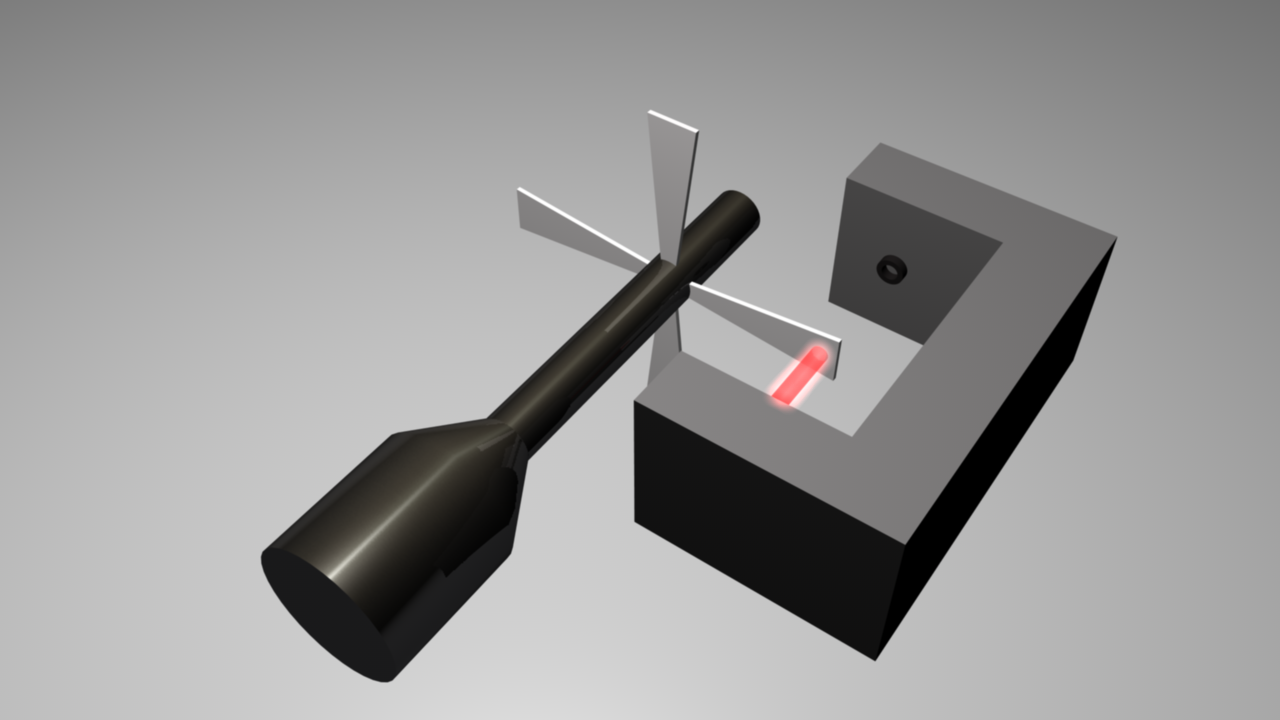
\includegraphics[scale=0.2]{./Graphics/Wheelspeed_D}
\caption{3D model af sensoren}
\label{wheelspeed3D}
\end{figure}

Efter test er der sat flere blade på viften da for at præcist at kunne bruge målingerne fra sensoren krævede det en højere opløsning. Dette fås ved at tilføje flere blade til viften så vi får flere pulses pr. omdrejning af aksen. Der er således nu så 4 blade på viften hvilket giver os 4 pulse pr. akse omdrejning. Dette svarer til 16,8 pulses pr. hjul omdrejning. \\
Se afsnit \ref{beregn_gearing} for udregningen af gearingen. \\
Dette giver en opløsning der er 4 gange bedre, end kun at have 1 vifte. \\
For bedre opløsning kunne der sættes flere vifter på, men kommer der for mange vifter på, vil det dog blive svært for sensoren at aflæse vifterne da deres mellemrum til sidst vil blive meget småt. Jo flere vifter der kommes på, jo sværere bliver det også at bygge ringen med vifterne. \\

Der bliver i dette tilfælde valgt at have 4 vifter da det kunne bygges forholdsvis let og det giver en opløsning der er høj nok til hvad vi ønskede. Ved blot 1 vifte kørte vi 2cm per omdrejning. Da vi ved hjulet kører 0,2381 omgange pr. motor omdrejning så kan længden den kører mellem hver puls udregnes ved at multiplicerer hjul omdrejninger med hjulets omkreds:
\begin{align*}
0,2381*8,5 = 2,02 cm
\end{align*}
Dette er ikke ret præcist da vi så kun kan aflæse længden/farten i intervaller af 2cm. Det blev så sat 4 vifter på og dette giver en præcision på:
\begin{align*}
(0,2381/4)* 8,5 = 0,51cm
\end{align*}
Dette er markant bedre da den nu kun kører 0,51cm før den får en puls og udregner længde og hastighed. Så der fås flere mindre intervaller der kan tjekkes og reageres på. \\ 

Som det kan ses på tegningen af kredsløbet i figur \ref{wheelspeedTegning} så er der sat nogle modstande og en kondensator på sensorens kredsløb. \\

\begin{figure}[h!]
\center
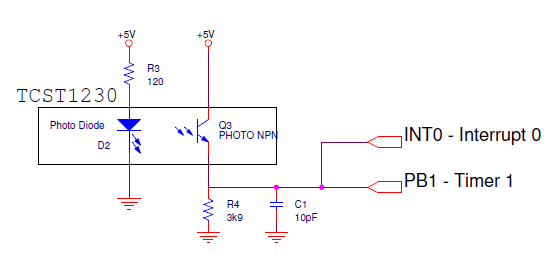
\includegraphics[scale=0.65]{./Graphics/TCST1230}
\caption{Kredsløbet til TCST1230 Sensoren}
\label{wheelspeedTegning}
\end{figure}

Modstanden R3 i figur \ref{wheelspeedTegning} er der for at sørge for at strømmen over dioden D2 ikke bliver højere end den kan tåle. Dioden kan nemlig kun klarer 30mA ifølge databladet. \todo{indsæt datablad}\\

Modstanden R4 virker som en pulldown modstand der sørger for at hive signalet langt nok ned, når fototransistoren ikke modtager lys, så der er logisk lavt signal. \\

Kondensatoren C1 benyttes til at sorterer små signaler fra. Hvis signalet ”hopper” frem og tilbage ved en overgang fra logisk lavt til logisk højt vil kondensatoren tage de små hurtige skift og sorterer dem fra. På denne måde fjernes en del af støjen.  
Der blev gennem oscilloskop observeret pral på sensoren ved TTL signal behandling. Der var benyttet en forkert metode til at opbygge sensoren på. Der var anvendt en struktur som forårsagede at diode spændingen over fototransistoren ikke kunne komme under 0.6V. Der blev derfor udarbejdet en anden struktur som set i databadet s. 3. \todo{TCST1230 s. 3} Modstanden benyttet til dioden blev udregnet vha. Ohms lov og ved at sætte strømmen lig 30mA. Dette resulterede i en modstand for R3 på 120 Ohm. \\

R4, som er pulldown modstanden, blev beregnet ved at kigge på figur 8 i databladet \todo{indsæt datablad}. Her blev modstanden udregnet til ca. 4K Ohm. Der anvendes her en 3.9K Ohm modstand \\

\subsubsection{Fart Software}
\label{fartmål_software}
Sensorens output er sat på ”PB1” og ”PD3” som går til ”Timer1” og ”INT0” i micro-controlleren. Så hver gang den får en puls så bliver timeren og interruptet triggeret. Timeren bliver benyttet til at finde længden den har kørt. Dette er beskrevet i afsnit \ref{afstandmål_software}. \\

Interruptet benyttes sammen med Timer0 til at finde farten. Timer 0 er sat op så den inkrementer hvert 0.000064 sekund. Hvilket svarer til den inkrementerer hvert 64. mikrosekund. Dette er sat ved at bruge en prescale på 1024. Da clock frekvensen på micro-processoren er 16MHz udregnes det således: \\
\begin{align*}
1/(16 000 000 / 1024) = 0,000064 sek = 64 mikrosekunder 
\end{align*}

Dette bruges for at finde tiden mellem pulses som kan benyttes som udtryk for farten. Timeren er ligeledes sat op så hvis der er overflow i Timer0 så kaldes et andet interrupt der blot nulstiller timeren og den fortsætter så. \\

Flowdiagrammet i figur \ref{fart_chart} viser processen hver gang Interruptet bliver kaldt. Hvilket sker hver gang sensoren sender en puls. \\

\begin{figure}[h!]
\center
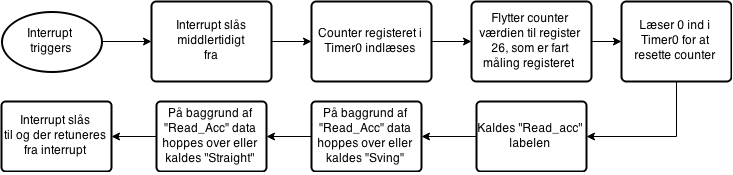
\includegraphics[scale=0.65]{./Graphics/fart_chart}
\caption{Flowchart af softwaren til måling af farten}
\label{fart_chart}
\end{figure}

Der slåes først interrupts fra globalt, for at dette interrupt ikke bliver afbrudt af et andet interrupt. Herefter indlæses den værdi tælleren er nået til. Denne værdi gemmes i registeret R26, som er vores ”målt fart” register. Så ligges der 0 ind i Timer0, for at nulstille den. På den måde får vi hvor mange gange der er gået 64 mikrosekunder på 1 puls. F.eks. hvis der går 10 optællinger mellem timer puls, så har bilen farten: 7,9 m/s. \\
Dette kan ses i lookup table i afsnit \todo{henvis til lookup table og sørg for table har korrekte enheder.}

Inden interruptet sluttes kaldes nogle labels der benyttes til at bestemme hvor på banen den er. Disse er beskrevet i afsnit XX. \todo{indsæt afsnit label} \\

Til sidst så slås interrupts til igen og der returneres til der koden var nået til, indtil næste interrupt bliver kaldt.  

\end{document}